\documentclass[a4paper,11pt]{article}
\usepackage[utf8]{inputenc}
\usepackage{graphicx}
\usepackage[spanish,es-nodecimaldot]{babel}
\usepackage[intlimits]{amsmath}
\usepackage{amsfonts}
\usepackage{subcaption}
\usepackage{booktabs} % Para las tablas
%\usepackage{ctable}   % para las captions de las tablas
\usepackage{placeins} % para evitar mezclar floats entre secciones
\usepackage{rotating}   % Para poner una tabla apaisada
\usepackage[table]{xcolor} % para colorear tablas
\usepackage{multirow}		% para agrupar filas
\usepackage{float}		% Habilita la opción H para fijar los floats

\usepackage{enumitem} % Para cambiar el label de enumerate fácilmente
\usepackage{textcomp} % Para el símbolo ¢ centavos
%---------------------- Marca de agua -------------------

% \usepackage{tikz}                       % Para que sea transparente en todos lados
% \usepackage[printwatermark]{xwatermark} % Para poner una marca de agua
% \newsavebox\mybox
% \savebox\mybox{\tikz[color=black,opacity=0.15]\node{RESERVADO};}
% \newwatermark*[allpages,angle=55,scale=9,xpos=-25,ypos=15]{\usebox\mybox}

%--------------------- Fin marca de agua ---------------

\usepackage[bottom]{footmisc} % para que las notas al pie queden abajo de la pägina aún cuando haya un espacio en blanco en la hoja.

\usepackage{hyperref}
\hypersetup{
    colorlinks = false,                                    % false:boxedlinks ; true:coloredlinks
    pdfborder = {0 0 0}
}

\usepackage{natbib}                                     % Para configurar la bibliografíaa
\setcitestyle{numbers,open={[},close={]},citesep={,}}   % Formato en que aparecen las citas en el documento
%\renewcommand\bibsection{\section{REFERENCIAS}}         % Renombra la bibliograf�a como REFERENCIAS y la pone en la TOC
\renewcommand\bibsection{\subsection{Documentación Aplicable}}         % Renombra la bibliograf�a como REFERENCIAS y la pone en la TOC

%\usepackage{babelbib}           % Para poner la bibliografía en español %(usando algún estilo de este paquete)

\usepackage[3autores, 3revisores, liberado]{itecnea}  
%\usepackage[3autores, 3revisores]{itecnea}  

\graphicspath{{src_figs/}}           % Define la ubicación de la carpeta donde están todas las imágenes


\newcommand{\E}[3]{$ #1 {\scriptstyle{\times}}10^{\text{#2}#3}$}

%%-----Información relevante para completar la carátula
\titulo{Ejemplo.}
\gerencia{GERENCIA XXXX}
\documento{INFORME}
\codigo{IN-EN-XXX}
\revision{0}
\autor{P. Bellino}
\coautoruno{X. XXX}
\coautordos{X. XXX}
\revisoruno{X. XXX}
\revisordos{X. XXX}
\revisortres{X. XXX}
\calidad{X. XXX}
%\calidad{\vspace{-5em} No utilizado por confidencialidad}
\aprobo{X. XXX}
% Información sobre las revisiones
\RevCeroNum{0}
\RevCeroDate{21/07/2025}
\RevCeroMod{Versión original}

%%-----Fin de la información para la carátula----------


%%-----Los objetivos y alcances se ponen en la carátula, pero entran como secciones del documento
%%-----La numeración queda de forma continua con el resto de las secciones.

\objetivo{%
  XXXXX.
}%

\resumen{%
Instalación del XXX.
}%
%%-----Fin de objetivos y alcances

\setcounter{tocdepth}{2}	% Hasta qué cosas se incluyen en la TOC

%%-----Comienzo formal del documento

\begin{document}

\renewcommand\tablename{Tabla}  % Pone "Tabla" en lugar de "Cuadro" cuando aparece una tabla.

\maketitle

\pagestyle{fancy}           % Para el resto de las páginas que ponga el encabezado definido en itecnea.sty

\renewcommand{\contentsname}{INDICE}
\tableofcontents

\newpage

\section{ABREVIATURAS Y DEFINICIONES} 

\subsection{Abreviaturas}\label{sec:abrev}

\renewcommand{\arraystretch}{1.2} % Separa un poco entre líneas (default=1)
\begin{tabular}{p{2.5cm} p{12.5cm}}

$\alpha_c$      & Constante de evolución de los neutrones instantáneos en estado crítico \\
$T_{sal}$       & Temperatura de salida del núcleo\\
$V^f_{M5}(t)$   & Voltaje $V_{M5}(t)$ luego de ser pasado por el filtro pasa-bajos  \\
\end{tabular}

\subsection{Definiciones}

\renewcommand{\arraystretch}{1}	% Vuelvo al valor por default
\begin{tabular}{p{2.5cm} p{12.5cm}}

BC   	& Barra de control \\
SPR     & Sistema primario de refrigeración \\
SEAD    & Sistema Electrónico de Adquisición de Datos \\
\end{tabular}


\newpage

\section{REFERENCIAS}

\subsection{Antecedentes}

\begin{itemize}
  \item XXXX
\end{itemize}

\bibliography{biblio}
\bibliographystyle{unsrtnat_pablo}
%\bibliographystyle{babunsrt} % un estilo posible para que aparezca en español (¿con babelbib?)

\subsection{Documentación Afectada}
No aplicable.

%\newpage
\setlength{\parskip}{0.3cm plus1mm minus1mm}


\section{RESPONSABILIDADES}

El presente documento es responsabilidad.
 
\section{DESARROLLO}

\subsection*{Resumen}

Con el objetivo de 

\subsection{Introducción}


\subsubsection{Técnica de ruido neutrónico}

La corriente de una cámara de ionización compensada ubicada cerca del núcleo de un reactor nuclear puede ser descripta,  como:


\subsection{Descripción}
Se utilizó sólo una cámara (CI1) para la estimación de potencia por ruido neutrónico.
El esquema simplificado del sistema de medición utilizado puede observarse en la Figura.


\begin{figure}[H]
  \centering
    \captionsetup{width=16cm}
    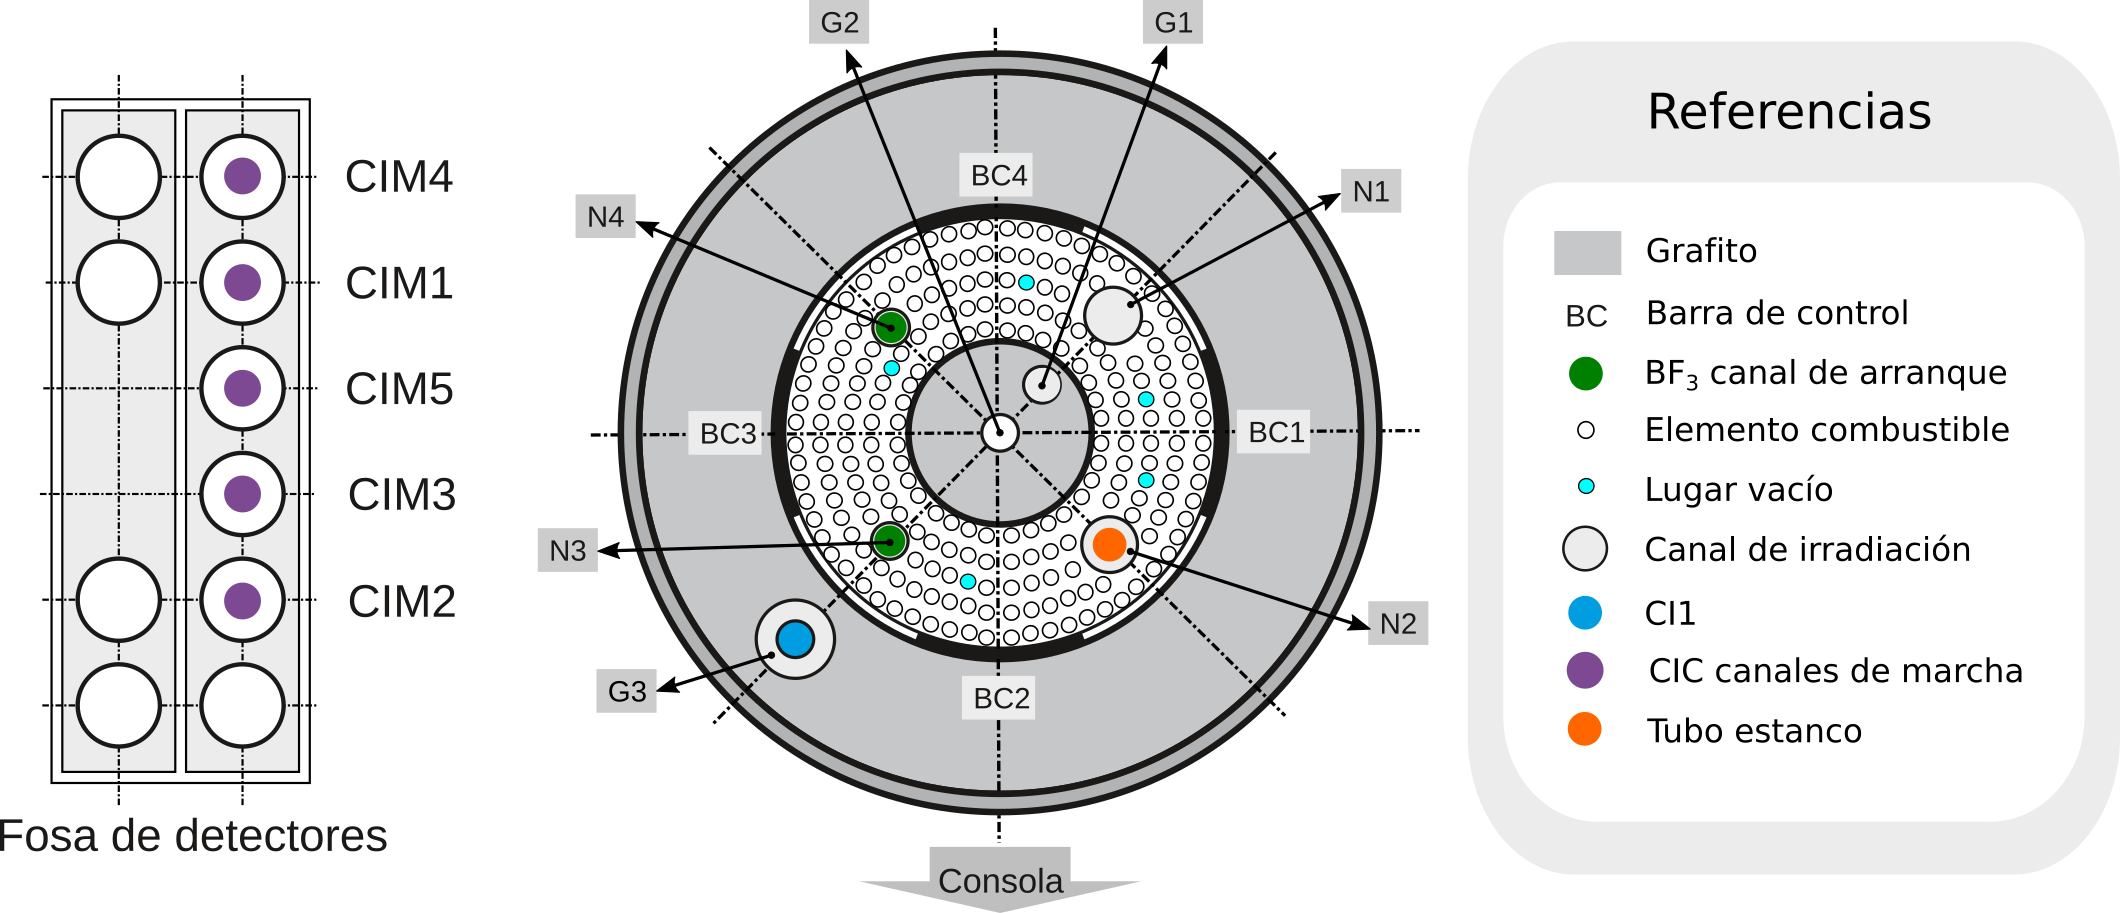
\includegraphics[width=17.0cm]{ra1_superior.png} \\
    \caption{Vista superior del núcleo del RA-1.}\label{fig:ra1_superior}
  \end{figure}   

\subsection{Equipos e instrumental}

\subsubsection*{Sistema de medición de ruido neutrónico}

\begin{enumerate}
  \item Cámara de ionización compensada, modelo CIC41.
\end{enumerate}


\subsection{Materiales e insumos}

No aplicable.

\subsection{Software}

XXXXX

\subsection{Condiciones ambientales}

XXXXX

%\FloatBarrier

\section{RESULTADOS}

XXXXXX

\subsubsection{Observaciones}

\begin{enumerate}[label=\alph*)]

  \item Los valores de $\alpha_c$ obtenidos para cada serie están dentro del rango esperado de acuerdo al análisis estadístico efectuado en con datos del núcleo 5 entre los años 1999 y 2016:


\end{enumerate}


\section{CONCLUSIONES}

Se realizaron mediciones 

%\newpage

\section{REGISTROS}


Todos los archivos utilizados para la confección de este informe se encuentran en.

\newpage

\section{ANEXOS}

\renewcommand{\theequation}{\thesubsection.\arabic{equation}}
\setcounter{equation}{0}  % reset counter
\renewcommand{\thetable}{\thesubsection.\arabic{table}}
\setcounter{table}{0}  % reset counter
\renewcommand{\thefigure}{\thesubsection.\arabic{figure}}
\setcounter{figure}{0}  % reset counter

\renewcommand{\thesubsection}{\Alph{subsection}}

\subsection*{Agradecimientos}

\vspace{-1em}
Se agradece a.

\subsection{Registro de mediciones}\label{sec:reg_med}

\begin{table}[H] 
	 \begin{center} 
		 % Se necesita el paquete 'array' para modificar con \begin{tabular}{>{$}c<{$}} 
		 % Usar \begin{sidewaystable} para apaisar 
		 \begin{tabular}{ >{$}c<{$} >{$}c<{$} >{$}c<{$} >{$}c<{$} >{$}c<{$} >{$}c<{$} >{$}c<{$} >{$}c<{$}}
			 \toprule 
                 \text{Nivel} & \text{Medición} & BW\,[Hz] & I_1\,[A] & I_{M5}\,[A] & BC3 [\%] & T_{en} [^\circ C] & T_{sal} [^\circ C] \\ 
			 \midrule 
			 \multirow{4}{*}{$1$} & 1 & 200 & 2.61(3) \times 10^{-6} & 1.74(5) \times 10^{-10} & \multirow{4}{*}{$44.1$} &\multirow{4}{*}{$19.2$} & \multirow{4}{*}{$18.6$} \\
			                    & 2 & 200 & 2.59(3) \times 10^{-6} & 1.73(5) \times 10^{-10} &                    &                   &                    \\
			                    & 3 & 40 & 2.60(3) \times 10^{-6} & 1.74(5)  \times 10^{-10} &                    &                   &                    \\
			                    & 4 & 40 & 2.60(3) \times 10^{-6} & 1.74(5)  \times 10^{-10} &                    &                   &                    \\ \midrule
			 \multirow{4}{*}{$2$} & 5 & 200 & 7.76(8) \times 10^{-6} & 5.3(1)  \times 10^{-10} & \multirow{4}{*}{$44.1$} &\multirow{4}{*}{$19.4$} & \multirow{4}{*}{$19.2$} \\
			                    & 6 & 200 & 7.77(9) \times 10^{-6} & 5.3(1)  \times 10^{-10} &                    &                   &                    \\
			                    & 7 & 40 & 7.8(1) \times 10^{-6} & 5.3(1)    \times 10^{-10} &                    &                   &                    \\
			                    & 8 & 40 & 7.8(1) \times 10^{-6} & 5.3(1)    \times 10^{-10} &                    &                   &                    \\ \midrule
			 \multirow{4}{*}{$3$} & 9 & 200 & 2.49(3) \times 10^{-5} & 1.68(5) \times 10^{-9}  & \multirow{4}{*}{$44.2$} &\multirow{4}{*}{$19.6$} & \multirow{4}{*}{$19.5$} \\
			                    & 10 & 200 & 2.55(3) \times 10^{-5} & 1.73(5)\times 10^{-9}  &                    &                   &                    \\
			                    & 11 & 40 & 2.56(3) \times 10^{-5} & 1.73(5) \times 10^{-9}  &                    &                   &                    \\
			                    & 12 & 40 & 2.60(5) \times 10^{-5} & 1.76(6) \times 10^{-9}  &                    &                   &                    \\ \midrule
			 \multirow{4}{*}{$4$} & 13 & 200 & 7.84(8) \times 10^{-5} & 5.4(1) \times 10^{-9}  & \multirow{4}{*}{$44.4$} &\multirow{4}{*}{$19.9$} & \multirow{4}{*}{$19.9$} \\
			                    & 14 & 200 & 7.79(8) \times 10^{-5} & 5.3(1) \times 10^{-9}  &                    &                   &                    \\
			                    & 15 & 40 & 7.74(8) \times 10^{-5} & 5.3(1)  \times 10^{-9}  &                    &                   &                    \\
			                    & 16 & 40 & 7.8(1) \times 10^{-5} & 5.3(1) \times 10^{-9} \\ 
			 \bottomrule 
		 \end{tabular} 
		 \caption{Corrientes y características.}
		 \label{tb:mediciones_ruido} 
	 \end{center} 
\end{table}


\end{document}
%%-----Fin del documento--------- 
